\documentclass[12pt]{extarticle}

%%%% paramètres généraux et commande prédéfinies
%%%% french character
\usepackage[french]{babel}
\usepackage[T1]{fontenc}
\usepackage[utf8]{inputenc}

%%%% useful packages
\usepackage[a4paper, left=1.3cm, right=1.3cm, top=2.2cm, bottom=2.3cm]{geometry}
\usepackage{subcaption} % for figure caption
\usepackage{graphicx} % image
\usepackage{tabularx} % table
\usepackage[table]{xcolor} % color in table
\usepackage{amsmath} % math
\usepackage{amssymb} % bold math
\usepackage{wasysym} % integral
\usepackage[many]{tcolorbox} % colored box
\usepackage{fancyhdr} % headers
\usepackage{enumitem} % for bullet in itemize
\usepackage[colorlinks=true,linkcolor=black,citecolor=black,filecolor=black,urlcolor=black]{hyperref} % for link
\usepackage{accents} % for complex notation
\usepackage[european, straightvoltages, RPvoltages]{circuitikz} % for electronic circuit
\usepackage{multicol} % to use several columns
\usepackage{fontawesome} % awesome icons
\usepackage{ifthen} % for loop and boolean in commands
\usepackage{pdfpages} % to include pdf
\usepackage{wrapfig} % to wrap text around figures
\usepackage{chemfig} % to draw chemistry formula
\usepackage{multirow} % for vertically merged cells
\usepackage{makecell} % to format cell in tables
\usepackage{physics} % for derivatives, braket, etc.
\usepackage{esvect} % for large vectors
\usepackage{listings} % for code
\usepackage{dashundergaps} % for automatic text to fill
\usepackage{tabularray} % for better tables
% dyslexia friendly font (need to be compiled in xetex)
%\usepackage{fontspec}
%\setmainfont{OpenDyslexic}


%%%% settings
\setlength{\parskip}{0cm}
\setlength{\parindent}{0cm}
\renewcommand{\baselinestretch}{1}
\setcounter{tocdepth}{2}


%%%% tikz configuration
\usetikzlibrary{babel}
\tikzset{>=latex}


%%%% header
\renewcommand{\headrulewidth}{0.4pt}
\setlength{\headheight}{22.50113pt}


%%%% Table
\renewcommand{\tabularxcolumn}[1]{m{#1}}
\setlength{\extrarowheight}{8pt}


%%%% Chemfig configuration
\setchemfig{
  atom sep=20pt,
  bond style={line width=1pt},
  angle increment=30
}


%%%% dashundergaps configuration
\dashundergapssetup{
  gap-numbers = false,
  gap-format = dot,
  gap-widen,
  gap-extend-percent
}
%% Format A5
% \geometry{a5paper}
%% Pour indiquer le barême dans une correction
\geometry{right = 2.7cm}


%%%% Mode élève (commenté) ou prof (décommenté)
\modeCorrection
%%%% pour l'en-tête
\renewcommand{\annee}{2023-2024}
\renewcommand{\etablissement}{Lycée Jean Moulin}


%%%% TP
\begin{document}
  %%%% tube à essai de sang
\newcommand{\tubeEssaiSang}[1]{
  \begin{subfigure}{0.1\linewidth}
    \centering
    \begin{tikzpicture}
      \tkzBasTubeEssai{#1}{0.25}{0}{0.75}{0.1}
      \tkzTubeEssai{0.25}{1.5}{0.1}
    \end{tikzpicture}
    \caption{}
  \end{subfigure}
}

%%%% Tube à essai de sang centrifugé
\newcommand{\tubeEssaiSangC}[3]{
  \centering
  \begin{tikzpicture}
    \tkzBasTubeEssai{rougeSombre!75!white}{0.5}{0}{#1}{0.1}
    \tkzPhaseTubeEssai{gray!10!white}{0.5}{#1}{#2}{0.1}
    \tkzPhaseTubeEssai{jauneClair!75!white}{0.5}{#2}{#3}{0.1}
    \tkzLegende{Plasma}{0.5}{#3 - 0.5}{2}
    \tkzLegende{Globules blancs}{0.5}{#2-0.08}{2}
    \tkzLegende{Globules rouges}{0.5}{-0.1}{2}
    \tkzTubeEssai{0.5}{#3 + 1}{0.1}
  \end{tikzpicture}
  \caption{}
}


%%%%
\newcommand{\VEth}{V_\text{éth}}
\newcommand{\mEth}{m_\text{éth}}
\newcommand{\rhoEth}{\rho_\text{éth}}
\newcommand{\cEth}{c_\text{éth}}
\newcommand{\COeq}{kg\chemfig{CO_2}e\;}
  %%%% Seconde
  %% Diagnostiques
  % %%%% début de la page
\newpage
\enTete{Corps purs et solutions}{1}

\nomPrenomClasse

%%%% titre
\titre{Changement d'état et solution}

\chevron {\large L'objectif de cette interrogation \textbf{non notée} est d'évaluer où vous en êtes en physique-chimie.}

%%%% question
\exo{Quels sont les 3 états de la matière ?}{0}
\vspace*{-0.3cm}
\begin{qcm}
  \item Air, terre, feu.
  \item Solide, mou, visqueux.
  \item Solide, liquide, gaz.
\end{qcm}

\exo{Cocher les phrases qui sont vraies :}{0}
\vspace*{-0.3cm}
\begin{qcm}
  \item L'eau est une espèce chimique liquide à température ambiante.
  \item L'eau a une masse volumique de $1000 \unit{g.cm^{-3}}$
  \item L'eau a une masse volumique de $1 \unit{kg.L^{-1}}$
\end{qcm}

\exo{L'eau salée est :}{0}
\vspace*{-0.3cm}
\begin{qcm}
  \item Un mélange homogène.
  \item Un mélange hétérogène.
  \item Une solution.
\end{qcm}

\exo{L'eau et l'huile :}{0}
\vspace*{-0.3cm}
\begin{qcm}
  \item Forment un mélange homogène.
  \item Forment un mélange hétérogène.
  \item Sont deux solutions miscibles.
  \item Ne sont pas deux solutions miscibles.
\end{qcm}

\exo{Une fusion est :}{0}
\vspace*{-0.3cm}
\begin{qcm}
  \item Le passage de l'état solide à l'état liquide.
  \item Le passage de l'état gazeux à l'état liquide.
  \item Le passage de l'état liquide à l'état solide.
\end{qcm}

\newpage
\exo{Comment s'appelle le passage d'un état liquide à un état gazeux ?}{1}

\exo{Légender le schéma suivant :}{0}
\vspace*{-0.3cm}
\begin{center}
  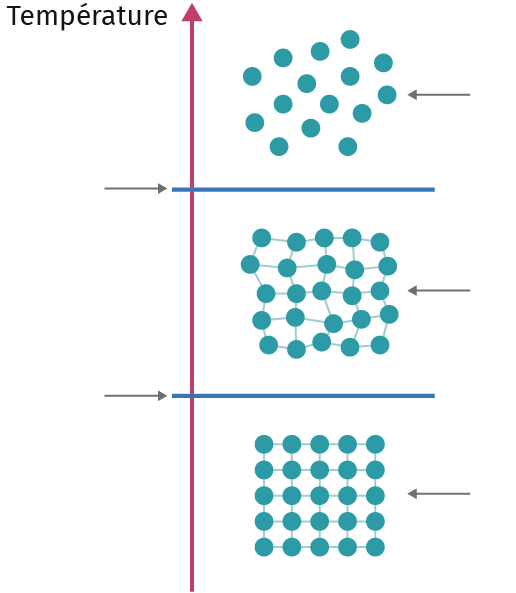
\includegraphics[width=0.6\linewidth]{evaluations/changement_etat.png}
\end{center}

\exo{Un fil de cuivre est :}{0}
\vspace*{-0.3cm}
\begin{qcm}
  \item Un corps pur.
  \item Un mélange.
  \item Une solution.
\end{qcm}
  % %%%% début de la page
\newpage
\enTete{Mouvement et interactions}{2}

\nomPrenomClasse

%%%% titre
\vspace{8pt}
\chevron L'objectif de cette interrogation \textbf{non notée} est d'évaluer où vous en êtes en physique-chimie.

%%%% question
%
\exo{Indiquer l'unité qui correspond à une vitesse.}{0}
\begin{qcm}
  \item Le mètre par seconde (m/s).
  \item Le kilomètre heure (km$\cdot$h).
  \item La seconde par mètre (s/m).
\end{qcm}

%
\exo{Une vitesse instantanée est représentée par une flèche qui porte 3 informations :}{0}
\begin{qcm}
  \item la distance, la direction et la durée.
  \item le sens, l'accélération et le nombre.
  \item la direction, le sens et la valeur.
\end{qcm}

%
\exo{Une observatrice observe depuis le quai un métro roulant à une vitesse constante.
Pour cette observatrice, le mouvement apparent du train est :}{1}

%
\exo{Un observateur est assis dans le métro roulant à une vitesse constante. 
Pour cet observateur, le mouvement apparent du train est :}{1}

%
\exo{Donner la formule de la force de pesanteur, le poids $P$, que l'on ressent sur Terre.}{1}

%
\exo{Indiquer la bonne expression de la force de pesanteur universelle $F_G$ entre deux objets de masse $m_A$ et $m_B$, séparés par une distance $d$.}{0}
\begin{qcm}
  \item $F_G = G \Frac{m_A m_B}{d^2}$
  \item $F_G = G m_A m_B$
  \item $F_G = G \Frac{m_A m_B}{d}$
\end{qcm}

%
\exo{Donner l'unité d'une force.}{1}
  %% Formative
  % %%%% début de la page
\newpage
\enTete{Corps purs et solutions}{1}

%%%%
\nomPrenomClasse

%%%% evaluation
\vspace*{6pt}
\begin{tableauCompetences}
  \centering RCO --
  Restituer ses connaissances.
  & & & &
  \\ \hline
  %
  \centering APP --
  Extraire une information
  & & & &
  \\ \hline
  %
  \centering REA --
  Réaliser un calcul.
  & & & &
\end{tableauCompetences}


%%%% questions
%
\exo{Un ensemble d'entités chimiques identiques est :\competence{RCO}}{0}
\vspace*{-4pt}
\begin{qcm}
  \item une espèce chimique.
  \item un corps pur.
  \item un mélange.
\end{qcm}

%
\exo{Définir un mélange.\competence{RCO}}{1}

%
\exo{Citer deux liquides \textbf{miscibles}.\competence{RCO}}{1}

%
L'acier doux est un alliage composé de fer (\chemfig{Fe}) et de carbone (\chemfig{C}).
Cet alliage est constitué d'une seule phase.
Un échantillon d'acier de masse $m = 1000 \unit{g}$ comporte une masse de fer $m_{\chemfig{Fe}} = 998 \unit{g}$ et une masse de carbone $m_{\chemfig{C}} = 2,\!00 \unit{g}$

%
\exo{Cet alliage est-il un mélange homogène ou hétérogène ?\competence{APP, RCO}}{1}

%
\exo{Écrire $m_{\chemfig{Fe}}$ et $m_{\chemfig{C}}$ en notation scientifique.\competence{APP, REA}}{1}

%
\exo{Calculer la proportion massique de fer et de carbone dans l'alliage.\competence{APP, REA}}{2}
  % %%%% début de la page
\newpage
\enTete{Corps purs et solutions}{1}

%%%%
\nomPrenomClasse

%%%% evaluation
\vspace*{6pt}
\begin{tableauCompetences}
  \centering RCO --
  Restituer ses connaissances.
  & & & & &
\end{tableauCompetences}


%%%% questions
%
\exo{Un ensemble d'entités chimiques identiques est : }{0}
\begin{qcm}
  \item une espèce chimique.
  \item un corps pur.
  \item un mélange.
\end{qcm}

%
\exo{Définir un mélange.}{1}

%
\vspace*{-12pt}
\exo{Deux liquides sont dits miscibles si ils}{0}
\begin{qcm}
  \item forment un mélange homogène.
  \item forment un mélange hétérogène.
\end{qcm}

%
\exo{Citer deux liquides \textbf{non-miscibles}.}{1}

%
\vspace*{-12pt}
\exo{Donner la formule de la masse volumique, en précisant le sens des symboles utilisés.}{3}

%
\vspace*{-12pt}
\exo{Une solution est :}{0}
\begin{qcm}
  \item Un mélange homogène.
  \item Un mélange hétérogène.
\end{qcm}

%
\exo{Donner le nom d'une solution dont le solvant est l'eau.}{1}

%
\vspace*{-12pt}
\exo{Donner la formule de la concentration massique, en précisant le sens des symboles utilisés.}{3}
  % %%%% début de la page
\newpage
\enTete{Mouvement et interactions}{2}

%%%%
\nomPrenom

%%%% evaluation
\vspace*{6pt}
\begin{tableauCompetences}
  \centering RCO 
  & Restituer ses connaissances.
  & & & &
\end{tableauCompetences}
\vspace*{8pt}

%%%% questions
%
\exo{Indiquer l'unité qui correspond à une vitesse.}{0}
\vspace*{-8pt}
\begin{qcm}
  \item Le mètre par seconde (m/s).
  \item Le kilomètre heure (km$\cdot$h).
\end{qcm}

%
\exo{Une vitesse est représenté par un vecteur qui porte 4 informations :}{0}
\vspace*{-8pt}
\begin{qcm}
  \item la position, la distance, la direction et la durée.
  \item le point, le sens, l'accélération et le nombre.
  \item le point d'application, la direction, le sens et la norme.
\end{qcm}

%
\exo{Une observatrice voit passer un métro roulant à une vitesse constante.
Pour elle le mouvement du métro est :}{1}

%
\exo{Un observateur est assis dans le métro roulant à une vitesse constante. 
Pour lui le mouvement du métro est :}{1}

%
\exo{Donner la formule du vecteur vitesse $\vv{v}_2$ d’un système au point $P_2$ entre les instants $t_1$ et $t_3$ :}{1}
  %% Fiche réussite
  % \enTeteFicheReussite{Chapitre 1 - Mélange et corps purs}

\begin{tableauConnaissancesSansExercices}
  Je sais la différence entre une espèce chimique et une entité chimique.
  & & & TP 1.1 \\
  % 
  Je sais la différence entre un corps pur et un mélange.
  & & & TP 1.1, TP 1.4 \\
  %
  Je sais décrire la composition d'un mélange avec les fractions volumiques et massiques.
  & & & activité 1.1 \\
  %
  Je connais la relation qui définit la masse volumique $\rho = m/V$.
  Je connais les unités et le sens de ces grandeurs. 
  Je sais calculer un volume, une masse ou une masse volumique avec cette relation.
  & & & TP 1.2, 1.3 et activité 1.2 \\
  %
  Je sais reconnaître si un échantillon est un corps pur constitué d'une seule espèce chimique ou s'il s'agit d'un mélange.
  & & & TP 1.1, TP 1.4, activité 1.1 \\
  %
  Je sais identifier un échantillon à partir de données physiques qui le caractérisent.
  & & & TP 1.2, TP 1.3 \\
  %
  Je sais identifier une espèce chimique à partir de tests chimiques caractéristiques.
  & & & TP 1.3 \\
  %
  Je connais le vocabulaire de la chromatographie sur couche mince : ligne de dépôt, couche mince, éluant, front de l'éluant, etc.
  & & & TP 1.4 \\
  % 
  Je sais analyser un chromatogramme pour identifier des espèces chimiques.
  & & & TP 1.4 \\
  % 
  Je sais analyser un chromatogramme pour reconnaitre un corps pur d'un mélange.
  & & & TP 1.4 \\
\end{tableauConnaissancesSansExercices}


\basDePageFicheReussite

\questionFicheReussite{3}

  % \enTeteFicheReussite{Chapitre 1 - Solutions}
\bigskip

\begin{tableauConnaissances}
  Je sais qu'une solution est un mélange homogène.
  Je sais qu'une solution est composé d'un solvant, l'espèce chimique majoritaire, et de un ou plusieurs solutés.
  & & & TP 4, cours p. 9 & 11 p. 48 \\
  %
  Je sais qu'on parle de solution aqueuse quand le solvant est l'eau.
  & & & TP 4 \& 5, cours p. 9 & \\
  %
  Je connais la formule de la concentration massique $c = m/V$.
  Je connais les unités et le sens de ces grandeurs.
  Je sais calculer une concentration massique, une masse ou un volume avec la formule.
  & & & TP 4 \& 5, cours p. 9, 10 & 14, 15 p. 49 \\
  %
  Je sais ce qu'est une dilution et une dissolution.
  Je connais le protocole pour réaliser une dilution.
  & & & TP 1, 4 \& 5, cours p. 10, 11 & 12, 16 p. 49 \\
  %
  Je sais qu'un dosage est une mesure de concentration.
  Je sais réaliser un dosage par étalonnage, en mesurant une grandeur proportionnelle à la concentration.
  & & & TP 4 \& 5, cours p. 12 & \\
\end{tableauConnaissances}

\basDePageFicheReussite{3}
  % \enTeteFicheReussite{3}{\sndMouv}
\bigskip

\begin{tableauConnaissances}
  % 
  Je sais que le mouvement dépend du référentiel choisi pour observer le mouvement. 
  & & & TP 3.1 et activité 3.1 \\
  %
  Je sais décrire le mouvement d'un système (trajectoire + évolution de son vecteur vitesse). Je sais reconnaître un mouvement rectiligne uniforme.
  & & &  Activité 3.1 \\
  %
  Je connais le modèle du point matériel.
  & & & Activité 3.1 \\
  % 
  Je sais calculer et tracer un vecteur vitesse à partir du vecteur déplacement et de l'écart de temps entre deux positions. 
  & & & TP 3.2 \\
  %
  Je sais qu'une force s'exprime en newton noté N et je sais représenter une force en terme de vecteurs, en faisant attention à son point d'application.
  & & & Activité 3.2, 3.3, 3.4, 3.5, 3.6 et 3.7 \\
  %
  Je sais quand deux forces se compensent.
  & & & Activité 3.3, 3.4 et 3.7 \\
  %
  Je connais les caractéristiques des forces suivantes : poids, réaction du support et forces de frottements.
  & & & Activité 3.2 et 3.6 \\
  %
  Je sais utiliser le principe d'inertie pour décrire les forces qui s'exercent sur un objet dont je connais le mouvement.
  & & & Activité 3.3, 3.4 et 3.7 \\
  %
  Je sais utiliser la contraposée du principe d'inertie pour décrire le mouvement d'un objet à partir des forces qui s'exercent sur l'objet.
  & & & Activité 3.3, 3.4 et 3.7 \\
  %
  Je sais sais vérifier l'homogénéité d'une relation entre deux grandeurs.
  & & & Activité 0.3 \\
  %
  Je sais calculer et utiliser des ordres de grandeurs.
  & & & Activité 0.3 \\
  %
\end{tableauConnaissances}

\basDePageFicheReussite

\coursFicheReussite
  % \enTeteFicheReussite{Chapitre 3 - Atome et ordre de grandeur}
\bigskip

\begin{tableauConnaissances}
  % 
  Je sais calculer et utiliser les puissances de dix.
  Je sais utiliser la notation scientifique.
  Je sais calculer un ordre de grandeur avec les puissances de dix.
  & & &  Activité 1 & Exercice 15, 16 \& 27 p. 81 \\
  %
  Je sais que la masse d’un atome est essentiellement contenue dans celle de son noyau.
  Je sais que le noyau est très petit devant la taille de l'atome.
  & & & Activité 2 & Exercice 9, 13 p. 81 \\
  %
  Je connais les charges électriques des électrons, neutrons et protons.
  J'ai compris pourquoi l'atome a une charge globale neutre.
  & & & Activité 2 \& 3 & \\
  %
  Je connais les composants d'un atome et de son noyau. 
  Je sais faire la différence entre électrons, protons, neutrons et nucléons.
  & & & Activité 3 & \\
  %
  Je peux déterminer la composition d'un atome à partir de sa notation symbolique \isotope{A}{Z}{X} et inversement.
  & & & Activité 3 & Exercice 7, 13 p. 81 \\
  %
  Je sais faire la différence entre les termes atome, ion, isotope.
  & & & Activité 3 & \\
  %
  Je sais que la description d'un atome est un modèle, dont l'évolution dépend d'observations expérimentales.
  & & & Activité 4 & Doc. p. 105 \\
  %
\end{tableauConnaissances}

\basDePageFicheReussite
\bigskip

\coursFicheReussite
  % \enTeteFicheReussite{Chapitre 3 - Cortège électronique, ions, molécules}
\bigskip

\begin{tableauConnaissances}
  %
  %Je sais que les électrons se structurent en couche (1, 2, 3) et sous-couche (s, p) autour du noyau.
  Je peux écrire la configuration électronique d'un atome en remplissant les sous-couches s et p dans le bon ordre.
  & & & Activité 5, 6 & \\
  %
  Je sais que les éléments chimiques sont rangées par colonne (famille) et par ligne (période) dans le tableau périodique.
  & & & Activité 6 & \\
  %
  Je peux identifier la couche externe d'un atome et combien d'électrons de valence s'y trouvent.
  & & & Activité 5, 6, 7, 8 & \\
  %
  Je sais repérer la famille des gaz nobles dans le tableau périodique.
  Je sais que leur couche externe pleine les rend très stables.
  & & & Activité 6, 7, 8 & \\
  %
  Je connais la règle du duet et de l'octet.
  Je peux les appliquer pour trouver quel ion stable peut être formé à partir d'un atome.
  & & & Activité 7 & \\
  %
  Je sais que les molécules sont composées d'atomes.
  Je sais que la stabilité d'une molécule est due aux électrons de valence partagés entre les atomes.
  & & & Activité 8 & \\
  %
  Je peux analyser un schéma de Lewis pour expliquer la stabilité d'une molécule.
  & & & Activité 8 & \\
  %
  Je sais qu'une espèce chimique est constitué d'un très grand nombre d'entités chimiques.
  Je sais ce que représente une mole.
  & & & Activité 9 & \\
  %
\end{tableauConnaissances}

\basDePageFicheReussite
\bigskip

\coursFicheReussite
  % \enTeteFicheReussite{Chapitre 4 - Ondes lumineuses et optique}
\bigskip

\begin{tableauConnaissancesSansExercices}
  %
  Je sais que la lumière est une onde électromagnétique.
  Je sais que la lumière peut être monochromatique ou polychromatique.
  & & & Activité 1 \\
  %
  Je connais les deux types de spectre d'émission et je sais les reconnaître.
  & & & TP 1 \\
  %
  Je sais qu'un corps chaud produit un spectre continu.
  Les propriétés de ce spectre dépendent de la température du corps chaud.
  & & & TP 1 \\
  %
  Je sais qu'un gaz atomique ou moléculaire excité produit un spectre de raies.
  Je sais que chaque élément chimique possède son propre spectre de raies qui permet de le reconnaître.
  & & & TP 1, activité 2 \\
  %
  Je sais repérer une raie sur un spectre en mesurant sa longueur d'onde.
  & & & TP 1, activité 2 \\
  %
  Je connais le vocabulaire de la réfraction et je sais lire les angles d'incidence et de réfraction à partir d'un schéma.
  & & & TP 2, activité 4 \\
  %
  Je sais appliquer la loi de Snell-Descartes pour calculer un indice de réfraction ou un angle.
  & & & TP 2, activité 4 \\
  %
  Je sais expliquer comment l'oeil parvient à faire l'image d'un objet.
  & & & Activité 3 \\
  %
  Je sais expliquer comment fonctionne une lentille convergente et je connais le vocabulaire pour la décrire (foyer image, foyer objet, centre optique).
  & & & TP 3, activité 3 \\
  %
  Je connais la formule du grandissement et je sais l'appliquer pour calculer la taille d'un objet ou d'une image.
  & & & TP 3, Activité 3 \\
  %
  Je sais expliquer pourquoi la lumière blanche est dispersée après avoir traversé un prisme.
  & & & Activité 4
  %
\end{tableauConnaissancesSansExercices}
\bigskip 

% \basDePageFicheReussite
% \coursFicheReussite
\questionFicheReussite{2}
  % \input{seconde/C7_transformations}
  % \input{seconde/C8_reaction_chimie}
  % \input{seconde/C9_signaux_capteurs}
  %% Sommative
  % \sujetA %%%% début de la page
\teteSndCorp
\setcounter{page}{1}

%%%%
\nomPrenomClasse

%%%%
\titreEvaluation{\sndCorp}

%%%% Compétences évaluées
\sousTitre{Compétences évaluées}

\begin{tableauCompetences}
  \centering RCO &
  Connaître le vocabulaire du cours et les relations importantes.
  & & & & \\
  %
  \centering APP &
  Extraire des informations d'un document.
  & & & &  \\
  %
  \centering VAL &
  Comparer des valeurs calculées avec des valeurs de références pour valider un raisonnement.
  & & & & \\
  %
  \centering REA &
  Réaliser un calcul en donnant le résultat en notation scientifique avec les bonnes unités.
  & & & & \\
\end{tableauCompetences}

\appreciation{4}


%%%% Exercice I
\vspace*{-20pt}
\titrePartie{Marais salant et pollution}

Les marais salants sont de grands bassin remplis par d'eau de mer, qui est riche en sel.
Le sel est du chlorure de sodium de formule brute \chemfig{NaCl}.

%
\question{
  Indiquer en justifiant si l'eau de mer est un corps pur ou un mélange.\competence{RCO, APP}
}{
  C'est un mélange, composé d'au moins deux espèces chimique : l'eau et le sel.
}{1}

Le soleil et le vent font s'évaporer l'eau de mer, mais le sel reste au fond des bassins. 
Après plusieurs étapes d'évaporation et de remplissage, la quantité de sel contenue dans l'eau des bassins devient très importante.
La masse volumique de l'eau salée augmente avec la quantité de sel.

\question{
  Rappeler la relation mathématique entre la masse volumique de l'eau salée $\rho$, sa masse $m$ et le volume $V$ qu'elle occupe.\competence{RCO}
}{
  \begin{equation*}
    \rho = \frac{m}{V}
  \end{equation*}
}{2}

Les productrices ou producteurs peuvent récolter le sel lorsque la masse volumique de l'eau salée dans un bassin est \textbf{supérieure} à $\rho_\text{récolte} = \qty{1,15}{\g/\ml}$.

\question{
  Une productrice de sel pèse \qty{50}{\ml} d'eau salée provenant d'un bassin et mesure une masse de \variationSujet{\qty{60}{\g}}{\qty{55}{\g}}.
  Calculer la masse volumique de l'eau salée dans ce bassin.\competence{REA}
}{
  $m_\text{eau salée} = \qty{60}{\g}$ et $V_\text{eau salée} = \qty{50}{\ml}$. Donc 
  \begin{equation*}
    \rho_\text{eau salée} = \frac{\qty{60}{\g}}{\qty{50}{\ml}} = \qty{1,2}{\g/\ml}
  \end{equation*}
}{2}

\question{
  Est-ce que la productrice peut récolter le sel dans ce bassin ? Justifier.\competence{VAL}
}{
  La masse volumique de l'eau du bassin est \variationSujet{supérieure}{inférieure} à celle nécessaire pour récolter, donc la productrice \variationSujet{peut}{ne peut pas} récolter le sel.
}{2}


Une ingénieure agronome réalise une inspection des marais salants en baie de somme.
Pour vérifier que des ions ne pollue pas les marais, elle prélève puis teste l'eau des bassins avec différentes espèces chimiques.
Un tableau récapitulatif des tests qu'elle peut réaliser est présenté ci-dessous

\begin{center}
  \begin{tableau}{| c | c | c |}
    Espèce utilisée & Ion recherché & Résultat d'un test positif \\
    Nitrate d'argent & \ionChlorure & Précipité blanc \\
    \SetCell[r = 3]{c} Hydroxyde de sodium & \ionCuivreII & Précipité bleu \\
    & \ionFerII & Précipité vert \\
    & \ionFerIII & Précipité rouille \\
    Chlorure de baryum & \ionSulfate & Précipité blanc \\
  \end{tableau}
\end{center}

\question{
  L'ingénieure commence par verser quelques gouttes de \variationSujet{chlorure de Baryum}{nitrate d'argent} dans un tube à essai contenant l'eau prélevée.
  Elle observe la formation d'un précipité blanc.
  Indiquer quel ion pollue le bassin, en justifiant.\competence{APP}
}{
   D'après le tableau, le \variationSujet{chlorure de baryum}{nitrate d'argent} a réagit avec les ions \variationSujet{sulfates}{chlorure} pour former un précipité blanc.
}{2}

\question{
  L'ingénieure veut réaliser des tests supplémentaires pour savoir si le bassin est aussi pollué par des ions Fer.
  Indiquer quel(s) réactif(s) elle doit utiliser et quel résultat permettrait de conclure à la présence d'ions Fer.\competence{APP}
}{
  Pour identifier la présence d'ions fer, l'ingénieure devra réaliser un test avec l'hydroxyde de sodium.
  Si elle voit apparaître un précipité vert, alors le bassin contient des ions Fer II.
  Si elle voit apparaître un précipité rouille, alors le bassin contient des ions Fer III.
  Si aucun précipité n'apparaît, le bassin n'est pas pollué.
}{4}


%%%% Exercice II
\vspace*{-20pt}
\titrePartie{Huile essentielle de \variationSujet{lavande}{menthe}}

Les huiles essentielles de \variationSujet{lavande}{menthe} sont obtenues par distillation des fleurs de \variationSujet{lavandes}{menthe}.
Les huiles essentielles sont riches en molécules odorantes.
On réalise une Chromatographie sur Couche Mince (CCM) afin d'identifier quelques espèces chimiques présentes dans cette huile essentielle.
Le chromatogramme obtenue après la montée de l'éluant est présenté ci-dessous.

\begin{figure}[!ht]
  \centering
  \variationSujet{
    \image{0.21}{images/chromato_lavande}
  }{
    \image{0.2}{images/chromato_menthe}
  }
  
  A : huile essentielle de \variationSujet{lavande}{menthe},
  B : \variationSujet{linalol}{menthol},
  C : \variationSujet{acétate de linalyle}{limonène}
  
  Chromatogramme.
\end{figure}

\numeroQuestion
Indiquer sur le chromatogramme où se trouvent la ligne de dépôt, la couche mince et le front de l'éluant.\competence{RCO}

\question{
  Justifier que l'huile essentielle de \variationSujet{lavande}{menthe} est un mélange.\competence{RCO, APP}
}{
  D'après le chromatogramme, le dépôt d'huile essentielle s'est divisé en trois tâches, c'est donc un mélange.
}{2}

\question{
  En comparant les hauteurs des tâches, indiquer quelles sont les espèces chimiques présentes dans l'huile essentielle de \variationSujet{lavande}{menthe}.\competence{RCO, APP, VAL}
}{
  Sur un chromatogramme, deux composés sont identiques s'ils sont montés à la même hauteur. 
  Sur le chromatogramme, on voit que la première tâche d'huile essentielle de \variationSujet{lavande}{menthe} est à la même hauteur que le \variationSujet{l'acétate de linalyle}{limonène} et que la seconde tâche est à la même hauteur que le \variationSujet{linalol}{menthol}.
  L'huile essentielle de \variationSujet{lavande}{menthe} est donc composée de \variationSujet{l'acétate de linalyle}{limonène} et de \variationSujet{linalol}{menthol}.
}{3}

\question{
  Peut-on identifier le troisième composé présent dans l'huile essentielle avec ce chromatogramme ?\competence{APP, VAL}
}{
  Non, car on n'a pas d'espèce chimique de référence pour comparer.
}{2}


%%%% Exercice III
\titrePartie{Étalon du kilogramme}

\begin{wrapfigure}[6]{r}{0.2\linewidth}
  \centering
  \vspace*{-40pt}
  \image{0.9}{images/standard_kilogram.jpg}
\end{wrapfigure}

Le kilogramme est l'unité de base de la masse dans le système international.
L'étalon qui \textbf{a servi à définir le kilogramme} jusqu'en mai 2019 est conservé par le Bureau International des Poids et Mesures (BIPM).
Ce prototype est un cylindre constitué d'un alliage de platine et d'iridium, de volume $V_\text{étalon} = \qty{47,191}{\cm\cubed}$ et de masse volumique $\rho_\text{étalon} = \qty{21,191}{\g/\cm\cubed}$.

\question{
  Sans calcul, indiquer la masse de l'étalon.\competence{APP}
}{
  L'étalon sert à définir le kilogramme.
  Sa masse est donc de \qty{1}{\kg} par définition.
}{1}

\question{
  Le prototype est composé de \qty{0,9}{\kg} de platine et de \qty{0,1}{\kg} d'iridium.
  Calculer la fraction massique de platine et d'iridium.\competence{REA, APP}
}{
  Pour le platine : $\qty{0,9}{\kg} / \qty{1}{\kg} = \qty{90}{\percent}$.
  Pour l'iridium : $\qty{0,1}{\kg} / \qty{1}{\kg} = \qty{10}{\percent}$
}{2}

\textit{Rappel :} la fraction massique d'une espèce dans un échantillon est la masse de l'espèce divisée par la masse totale de l'échantillon.
Par exemple pour le platine :
\begin{equation*}
  p_v(\text{platine}) = \frac{m_\text{platine}}{m_\text{étalon}}
\end{equation*}

\question{
  Historiquement, un premier cylindre avait été réalisé avec \qty{11,1}{\percent} d'iridium, qui a une masse volumique plus élevée que le platine.
  Sachant que son volume était identique à l'étalon actuel, indiquer si la masse de ce cylindre valait 1 kg et expliquer pourquoi il avait été rejeté par le BIPM.\competence{APP}
}{
  L'étalon actuel a précisément une masse de \qty{1}{\kg} avec \qty{10}{\percent} d'iridium.
  Le premier cylindre comportait $\qty{11,1}{\percent} > \qty{10}{\percent}$ d'iridium.
  Comme l'iridium a une masse volumique plus élevée, sa masse valait plus de \qty{1}{\kg}, d'où le rejet par le BIPM.
}{2}


\setcounter{sousSectionNum}{0}

%%%% Correction
\newpage
\vspace*{-36pt}
\titreSousSection{Ma correction (à faire après la correction du professeur)}

%%%% Tableau de correction élève
\begin{tblr}{
    row{1} = {couleurPrim!20}, hlines,
    colspec = {| X[-1, c] | X[2, c] | X[2, c] | X[2, c] |}
  }
  \textbf{Question} & 
  \textbf{L'erreur} &
  \textbf{Analyse de l'erreur} &
  \textbf{La correction} \\
  %
  \phantom{b} \vspace{55 pt} & & & \\
  \phantom{b} \vspace{55 pt} & & & \\
  \phantom{b} \vspace{55 pt} & & & \\
  \phantom{b} \vspace{55 pt} & & & \\
\end{tblr}


%%%% Bilan
\titreSousSection{Mon bilan après mon travail de correction}

%%%% Tableau bilan de la correction
\begin{tableau}{| X[c] | X[c] |}
  \textbf{Ce que je n'avais pas compris...} &
  \textbf{Ce que maintenant j'ai compris...} \\
  \phantom{b} \vspace{150 pt} & \\
\end{tableau}


%%%% Acquis
\titreSousSection{Mes acquis après mon travail de correction (à remplir par le professeur)}

\appreciation{2}
  % \sujetB %%%% début de la page
\teteSndCorp
\setcounter{page}{1}

%%%%
\nomPrenomClasse

%%%%
\titreEvaluation{\sndCorp}

%%%% Compétences évaluées
\sousTitre{Compétences évaluées}

\begin{tableauCompetences}
  \centering RCO &
  Connaître le vocabulaire du cours et les relations importantes.
  & & & & \\
  %
  \centering APP &
  Extraire des informations d'un document.
  & & & &  \\
  %
  \centering VAL &
  Comparer des valeurs calculées avec des valeurs de références pour valider un raisonnement.
  & & & & \\
  %
  \centering REA &
  Réaliser un calcul en donnant le résultat en notation scientifique avec les bonnes unités.
  & & & & \\
\end{tableauCompetences}

\appreciation{4}


%%%% Exercice I
\vspace*{-20pt}
\titrePartie{Marais salant et pollution}

Les marais salants sont de grands bassin remplis par d'eau de mer, qui est riche en sel.
Le sel est du chlorure de sodium de formule brute \chemfig{NaCl}.

%
\question{
  Indiquer en justifiant si l'eau de mer est un corps pur ou un mélange.\competence{RCO, APP}
}{
  C'est un mélange, composé d'au moins deux espèces chimique : l'eau et le sel.
}{1}

Le soleil et le vent font s'évaporer l'eau de mer, mais le sel reste au fond des bassins. 
Après plusieurs étapes d'évaporation et de remplissage, la quantité de sel contenue dans l'eau des bassins devient très importante.
La masse volumique de l'eau salée augmente avec la quantité de sel.

\question{
  Rappeler la relation mathématique entre la masse volumique de l'eau salée $\rho$, sa masse $m$ et le volume $V$ qu'elle occupe.\competence{RCO}
}{
  \begin{equation*}
    \rho = \frac{m}{V}
  \end{equation*}
}{2}

Les productrices ou producteurs peuvent récolter le sel lorsque la masse volumique de l'eau salée dans un bassin est \textbf{supérieure} à $\rho_\text{récolte} = \qty{1,15}{\g/\ml}$.

\question{
  Une productrice de sel pèse \qty{50}{\ml} d'eau salée provenant d'un bassin et mesure une masse de \variationSujet{\qty{60}{\g}}{\qty{55}{\g}}.
  Calculer la masse volumique de l'eau salée dans ce bassin.\competence{REA}
}{
  $m_\text{eau salée} = \qty{60}{\g}$ et $V_\text{eau salée} = \qty{50}{\ml}$. Donc 
  \begin{equation*}
    \rho_\text{eau salée} = \frac{\qty{60}{\g}}{\qty{50}{\ml}} = \qty{1,2}{\g/\ml}
  \end{equation*}
}{2}

\question{
  Est-ce que la productrice peut récolter le sel dans ce bassin ? Justifier.\competence{VAL}
}{
  La masse volumique de l'eau du bassin est \variationSujet{supérieure}{inférieure} à celle nécessaire pour récolter, donc la productrice \variationSujet{peut}{ne peut pas} récolter le sel.
}{2}


Une ingénieure agronome réalise une inspection des marais salants en baie de somme.
Pour vérifier que des ions ne pollue pas les marais, elle prélève puis teste l'eau des bassins avec différentes espèces chimiques.
Un tableau récapitulatif des tests qu'elle peut réaliser est présenté ci-dessous

\begin{center}
  \begin{tableau}{| c | c | c |}
    Espèce utilisée & Ion recherché & Résultat d'un test positif \\
    Nitrate d'argent & \ionChlorure & Précipité blanc \\
    \SetCell[r = 3]{c} Hydroxyde de sodium & \ionCuivreII & Précipité bleu \\
    & \ionFerII & Précipité vert \\
    & \ionFerIII & Précipité rouille \\
    Chlorure de baryum & \ionSulfate & Précipité blanc \\
  \end{tableau}
\end{center}

\question{
  L'ingénieure commence par verser quelques gouttes de \variationSujet{chlorure de Baryum}{nitrate d'argent} dans un tube à essai contenant l'eau prélevée.
  Elle observe la formation d'un précipité blanc.
  Indiquer quel ion pollue le bassin, en justifiant.\competence{APP}
}{
   D'après le tableau, le \variationSujet{chlorure de baryum}{nitrate d'argent} a réagit avec les ions \variationSujet{sulfates}{chlorure} pour former un précipité blanc.
}{2}

\question{
  L'ingénieure veut réaliser des tests supplémentaires pour savoir si le bassin est aussi pollué par des ions Fer.
  Indiquer quel(s) réactif(s) elle doit utiliser et quel résultat permettrait de conclure à la présence d'ions Fer.\competence{APP}
}{
  Pour identifier la présence d'ions fer, l'ingénieure devra réaliser un test avec l'hydroxyde de sodium.
  Si elle voit apparaître un précipité vert, alors le bassin contient des ions Fer II.
  Si elle voit apparaître un précipité rouille, alors le bassin contient des ions Fer III.
  Si aucun précipité n'apparaît, le bassin n'est pas pollué.
}{4}


%%%% Exercice II
\vspace*{-20pt}
\titrePartie{Huile essentielle de \variationSujet{lavande}{menthe}}

Les huiles essentielles de \variationSujet{lavande}{menthe} sont obtenues par distillation des fleurs de \variationSujet{lavandes}{menthe}.
Les huiles essentielles sont riches en molécules odorantes.
On réalise une Chromatographie sur Couche Mince (CCM) afin d'identifier quelques espèces chimiques présentes dans cette huile essentielle.
Le chromatogramme obtenue après la montée de l'éluant est présenté ci-dessous.

\begin{figure}[!ht]
  \centering
  \variationSujet{
    \image{0.21}{images/chromato_lavande}
  }{
    \image{0.2}{images/chromato_menthe}
  }
  
  A : huile essentielle de \variationSujet{lavande}{menthe},
  B : \variationSujet{linalol}{menthol},
  C : \variationSujet{acétate de linalyle}{limonène}
  
  Chromatogramme.
\end{figure}

\numeroQuestion
Indiquer sur le chromatogramme où se trouvent la ligne de dépôt, la couche mince et le front de l'éluant.\competence{RCO}

\question{
  Justifier que l'huile essentielle de \variationSujet{lavande}{menthe} est un mélange.\competence{RCO, APP}
}{
  D'après le chromatogramme, le dépôt d'huile essentielle s'est divisé en trois tâches, c'est donc un mélange.
}{2}

\question{
  En comparant les hauteurs des tâches, indiquer quelles sont les espèces chimiques présentes dans l'huile essentielle de \variationSujet{lavande}{menthe}.\competence{RCO, APP, VAL}
}{
  Sur un chromatogramme, deux composés sont identiques s'ils sont montés à la même hauteur. 
  Sur le chromatogramme, on voit que la première tâche d'huile essentielle de \variationSujet{lavande}{menthe} est à la même hauteur que le \variationSujet{l'acétate de linalyle}{limonène} et que la seconde tâche est à la même hauteur que le \variationSujet{linalol}{menthol}.
  L'huile essentielle de \variationSujet{lavande}{menthe} est donc composée de \variationSujet{l'acétate de linalyle}{limonène} et de \variationSujet{linalol}{menthol}.
}{3}

\question{
  Peut-on identifier le troisième composé présent dans l'huile essentielle avec ce chromatogramme ?\competence{APP, VAL}
}{
  Non, car on n'a pas d'espèce chimique de référence pour comparer.
}{2}


%%%% Exercice III
\titrePartie{Étalon du kilogramme}

\begin{wrapfigure}[6]{r}{0.2\linewidth}
  \centering
  \vspace*{-40pt}
  \image{0.9}{images/standard_kilogram.jpg}
\end{wrapfigure}

Le kilogramme est l'unité de base de la masse dans le système international.
L'étalon qui \textbf{a servi à définir le kilogramme} jusqu'en mai 2019 est conservé par le Bureau International des Poids et Mesures (BIPM).
Ce prototype est un cylindre constitué d'un alliage de platine et d'iridium, de volume $V_\text{étalon} = \qty{47,191}{\cm\cubed}$ et de masse volumique $\rho_\text{étalon} = \qty{21,191}{\g/\cm\cubed}$.

\question{
  Sans calcul, indiquer la masse de l'étalon.\competence{APP}
}{
  L'étalon sert à définir le kilogramme.
  Sa masse est donc de \qty{1}{\kg} par définition.
}{1}

\question{
  Le prototype est composé de \qty{0,9}{\kg} de platine et de \qty{0,1}{\kg} d'iridium.
  Calculer la fraction massique de platine et d'iridium.\competence{REA, APP}
}{
  Pour le platine : $\qty{0,9}{\kg} / \qty{1}{\kg} = \qty{90}{\percent}$.
  Pour l'iridium : $\qty{0,1}{\kg} / \qty{1}{\kg} = \qty{10}{\percent}$
}{2}

\textit{Rappel :} la fraction massique d'une espèce dans un échantillon est la masse de l'espèce divisée par la masse totale de l'échantillon.
Par exemple pour le platine :
\begin{equation*}
  p_v(\text{platine}) = \frac{m_\text{platine}}{m_\text{étalon}}
\end{equation*}

\question{
  Historiquement, un premier cylindre avait été réalisé avec \qty{11,1}{\percent} d'iridium, qui a une masse volumique plus élevée que le platine.
  Sachant que son volume était identique à l'étalon actuel, indiquer si la masse de ce cylindre valait 1 kg et expliquer pourquoi il avait été rejeté par le BIPM.\competence{APP}
}{
  L'étalon actuel a précisément une masse de \qty{1}{\kg} avec \qty{10}{\percent} d'iridium.
  Le premier cylindre comportait $\qty{11,1}{\percent} > \qty{10}{\percent}$ d'iridium.
  Comme l'iridium a une masse volumique plus élevée, sa masse valait plus de \qty{1}{\kg}, d'où le rejet par le BIPM.
}{2}


\setcounter{sousSectionNum}{0}

%%%% Correction
\newpage
\vspace*{-36pt}
\titreSousSection{Ma correction (à faire après la correction du professeur)}

%%%% Tableau de correction élève
\begin{tblr}{
    row{1} = {couleurPrim!20}, hlines,
    colspec = {| X[-1, c] | X[2, c] | X[2, c] | X[2, c] |}
  }
  \textbf{Question} & 
  \textbf{L'erreur} &
  \textbf{Analyse de l'erreur} &
  \textbf{La correction} \\
  %
  \phantom{b} \vspace{55 pt} & & & \\
  \phantom{b} \vspace{55 pt} & & & \\
  \phantom{b} \vspace{55 pt} & & & \\
  \phantom{b} \vspace{55 pt} & & & \\
\end{tblr}


%%%% Bilan
\titreSousSection{Mon bilan après mon travail de correction}

%%%% Tableau bilan de la correction
\begin{tableau}{| X[c] | X[c] |}
  \textbf{Ce que je n'avais pas compris...} &
  \textbf{Ce que maintenant j'ai compris...} \\
  \phantom{b} \vspace{150 pt} & \\
\end{tableau}


%%%% Acquis
\titreSousSection{Mes acquis après mon travail de correction (à remplir par le professeur)}

\appreciation{2}
  % \sujetA \input{seconde/sommative/E2_solution}
  % \sujetB \input{seconde/sommative/E2_solution}
  % \sujetA %%%% début de la page
\teteSndMouv


%%%% TODO : 
% Changer les questions sur le poids -> calcul poids sur Terre et sur ISS, comparaison des deux 
% Deux forces qui s'exercent sur la spationaute : P et Finertie
% Changer question inertie -> F = m * v * v / (RT + h) est-ce égal à P = m*g


%%%%
\nomPrenomClasse

%%%%
\titreEvaluation{\sndMouv}

%%%% Compétences évaluées
\pasCorrection{
  \sousTitre{Compétences évaluées}
  
  \begin{tableauCompetences}
    APP &
    Représenter une situation par un schéma simple.
    Extraire des informations d'un document.
    & & & & \\
    %
    REA &
    Réaliser un calcul en donnant le résultat en notation scientifique avec les bonnes unités.
    Calculer des ordres de grandeurs.
    & & & & \\
    %
    VAL &
    Comparer des valeurs calculées avec des valeurs de références pour valider un raisonnement.
    & & & & \\
    %
    ANA/RAI &
    Mener un raisonnement à partir de grandeur données ou calculées.
  \end{tableauCompetences}
}

\appreciation{3}



%%%%
\titreSection{Impesanteur}

%%
\vspace*{-10pt}
\begin{doc}{Station spatiale internationale (ISS)}{doc:E3_station_ISS}
  On lit parfois que les spationautes flottent dans les stations spatiales, car la gravité terrestre n'agit plus sur les spationautes.
  
  \begin{wrapfigure}{r}{0.4\linewidth}
    \vspace*{-30pt}
    \centering
    \image{0.8}{images/spationaute_ISS}
  \end{wrapfigure}
  
  On s'intéresse à la station spatiale internationale, notée ISS, en orbite circulaire autour de la Terre à une hauteur $h$.
  L'ISS a une vitesse constante $v$.

  \important{Données :}
  \begin{listePoints}
    \item $G = \qty{6,67e-11}{\newton\m\squared \per\kg\squared}$
    \item $\MTerre = \qty{5,97e24}{\kg}$
    \item $\RTerre = \qty{6,37e6}{\m}$
    \item $h = \qty{3,70e5}{\m}$
    \item $v = \qty{7,66e3}{\m\per\s}$
  \end{listePoints}
\end{doc}

%%
\numeroQuestion
  \label{exo:schema_ISS}
  Quel est le mouvement décrit par l'ISS dans le référentiel lié au centre de la Terre ?
  Faire un schéma faisant figurer l'ISS, la Terre et la trajectoire qu'elle décrit.\competence{APP}\correction{\points{3}}

\question{
  Dans la station les spationautes ont un poids $P = m \times \gISS$.
  Calculer la valeur de $\gISS$ sachant que
  \begin{equation*}
    \gISS =  G \times \dfrac{\MTerre}{(\RTerre + h)^2}
  \end{equation*}\competence{APP, REA}
}{
  \begin{equation*}
    \gISS
    = \qty{6,67e-11}{\newton\m\squared \per\kg\squared}
    \dfrac{\qty{5,97e24}{\kg}} {(\num{6,37e6} + \qty{3,70e5}{\m})^2}
    %
    = \qty{8,77}{\newton}
    \points{1,5}
  \end{equation*}
}{0}


\pasCorrection{\newpage}
\question{
  Comparer avec l'accélération de pesanteur terrestre $g = \qty{9,81}{\newton\per\kg}$.
  Peut-on vraiment dire que la gravité terrestre n'agit plus sur les spationautes au sein de l'ISS ?\competence{VAL, ANA/RAI}
}{
  $\gISS$ est presque égal à $g$, donc la gravité agit toujours fortement.
  \points{1}
}{0}

\question{
  \label{exo:calcul_poids_ISS}
  En sachant que $\gISS = \qty{8,77}{\newton\per\kg}$, calculer le poids d'une spationaute de masse $m = \qty{65}{\kg}$ dans l'ISS.\competence{REA}
}{
  \begin{equation*}  
    P = \qty{65}{\kg} \times \qty{8,77}{\newton\per\kg} = \qty{570}{\newton}
    \points{1,5}
  \end{equation*}
}{0}


%%
\begin{doc}{Force d'inertie d'entraînement}{doc:E3_force_inertie}
  Un système dans un référentiel en rotation est soumis à une force \important{relative} qui dépend du référentiel, qu'on appelle \important{force d'inertie d'entraînement} $\vv{F}_\inertie$ ou encore « force centrifuge ».

  Cette force a pour direction la \important{droite reliant le centre du cercle et le centre du système.}
  Son sens est dirigé \important{vers l'extérieur du cercle.}
  C'est cette force qui explique pourquoi les passagers d'une voiture dans un rond-point sentent leur corps attiré vers l'extérieur du rond-point.

  \begin{encart}
    \important{Rappel :} le principe d'inertie dit que tout objet immobile est soumis à des forces dont la somme est nulle.
  \end{encart}
\end{doc}

\question{
  Expliquer avec vos mot le principe d'inertie.\competence{COM}
}{
  Il faut exercer une force sur un objet pour changer son mouvement, par défaut les objets se déplacent en ligne droite.
  \points{3}
}{0}

\question{
  Dans le référentiel lié à l'ISS, la spationaute est immobile.
  En utilisant le principe d'inertie et en justifiant clairement, donner la norme de la force d'inertie d'entraînement $F_\inertie$ qui s'exerce sur la spationaute.\competence{APP, ANA/RAI}
}{
  Comme la spationaute est immobile, la somme des forces qui s'exercent sur elle est nulle et $F_\inertie = P = \qty{8,77}{\newton}$
  \points{2}
}{0}

\numeroQuestion
  Compléter le schéma de la question~\ref{exo:schema_ISS} en représentant les forces s'exerçant sur la spationaute dans le référentiel lié à l'ISS.\competence{APP, REA}\correction{\points{1}}


\question{
  La norme de la force d'inertie d'entraînement exercée sur la spationaute est
  \begin{equation*}
    F_\inertie = m \times \dfrac{v^2}{R}
    \label{eq:force_inertie}
  \end{equation*}
  où $v$ est la vitesse du référentiel et $R$ est la distance entre le centre de rotation du référentiel et le centre du système (donc $R = \RTerre + h$ ici). 
  Cette relation est-elle cohérente avec le principe d'inertie ?
  
  \textit{
    Prendre des initiatives et les écrire, même si le raisonnement n'est pas complet.
    Tout début de réflexion sera valorisé.
  }
  \competence{APP, REA, VAL, ANA/RAI}
}{
  On calcule la valeur de $F_\inertie$ :
  \begin{equation*}
    F_\inertie
    = \qty{65}{\kg} \times \dfrac{(\qty{7,66}{\m\per\s})^2}{\num{6,37e6} + \qty{3,70e5}{\m}}
    = \qty{565}{\newton}
  \end{equation*}
  On retrouve presque la même valeur qu'à la question 4, cette norme est donc cohérente avec le principe d'inertie.
  \points{3}
}{0}

%% Formulation officielle du BAC
% Le candidat est invité à prendre des initiatives et à présenter la démarche suivie, même si elle n'a pas abouti. La démarche est évaluée et nécessite d'être correctement présentée.
\pasCorrection{
  \begin{coupDePouce}
    Utiliser les données de l'énoncé pour calculer $F_\inertie$. 
    Comparer cette valeur avec celle obtenue à la question~\ref{exo:calcul_poids_ISS} et conclure.
  \end{coupDePouce}
}



%%%%
\titreSection{Ordre de grandeur et écologie}

\begin{doc}{Activités humaines et émission de gaz à effet de serre}{doc:E3_effet_serre}
  On va chercher à estimer l'impact de notre alimentation sur le climat, en comparant avec l'impact du secteur automobile.
  Pour cela on va estimer l'ordre de grandeur des émissions de gaz à effet de serre rejetés lors de la production de nos aliments.
  
  Pour mesurer l'impact sur le climat d'un produit, on utilise le kilogramme de dioxyde de carbone équivalent, noté \unit{\COeq}.
  \important{Plus ce nombre est élevé et plus un produit a un impact important sur le dérèglement climatique.}
  
  Par exemple, produire 1 kg de viande de mouton équivaut à l'émission de 39,72 kg de \chemfig{CO_2}, soit 39,72 \unit{\COeq} (voir tableau).
  Cette émission correspond à l'émission d'une voiture qui parcours 400 km.
  
  \begin{encart}
    \important{Rappel :} l'ordre de grandeur d'un nombre est la puissance de 10 la plus proche de ce nombre. 
    Par exemple l'ordre de grandeur de 70 est 100.
    L'ordre de grandeur de 4 est 1.
  \end{encart}
\end{doc}

\question{
  Donner un ordre de grandeur du nombre de repas (déjeuner et dîner) par an.
  \textbf{Rappel :} 1 an = 365 jours\competence{REA}
}{
  Avec 2 repas par jour en moyenne, on a $2 \times 365 = 730 \sim 1000$ repas par an en ordre de grandeur.
  \points{1,5}
}{0}

\question{
  \label{exo:ordre_alimentation}
  À l'aide du graphique ci-dessous, calculer en ordre de grandeur le \unit{\COeq} annuel d'un régime à base de viande.
  On considère qu'un-e français-e mange en moyenne \qty{0,1}{kg} de viande par repas.\competence{APP, REA, ANA/RAI}
}{
  \begin{wrapfigure}{r}{0.5\linewidth}
    \centering
    \vspace*{-16pt}
    \image{1}{images/emission_CO2_alimentation}
  \end{wrapfigure}
  En ordre de grandeur, la production de $\qty{1}{\kg}$ de mouton ou de poulet émet $\qty{10}{\COeq}$.
  Par an, un-e français-e mange en moyenne $\qty{0,1}{\kg} \times 1000 = \qty{100}{\kg}$ de viande par an.
  Les émissions par an seront donc
  % Par an, les émissions d'un-e français-e sera donc en moyenne les émissions pour $1\unit{kg}$ multipliée par la masse de viande mangée, soit
  \begin{equation*}
    \qty{100}{\kg} \times \qty{10}{\COeq/\kg} = \qty{e3}{\COeq}
  \end{equation*}
  On notera qu'un régime végétarien permet de diviser par 10 ses émissions liées à l'alimentation en ordre de grandeur !
  \points{2}
}{0}

\pasCorrection{
  \begin{center}
    \vspace{-12pt}
    \image{0.6}{images/emission_CO2_alimentation}
  \end{center}
  \vspace{-12pt}
}


\question{
  En moyenne, une personne qui possède une voiture en France émet en ordre de grandeur \qty{e3}{\COeq} en roulant \textbf{par an}.
  Comparer avec l'ordre de grandeur des émissions annuelle dues à l'alimentation.\competence{VAL}
}{
  On voit qu'en ordre de grandeur, les émissions liées à la voiture et à une alimentation à base de viande sont identiques.
  \points{1}
}{0}

\question{
  En réalité, sur une année le transport représente en moyenne \qty{2,4e3}{\COeq} et l'alimentation \qty{2,0e3}{\COeq}, sur un total annuel d'émission de \qty{8,0e3}{\COeq} pour une personne vivant en France.
  
  Est-ce que le chiffre de l'alimentation est cohérent avec l'ordre de grandeur estimé question~\ref{exo:ordre_alimentation} ?\competence{APP, VAL}
}{
  En ordre de grandeur $\qty{2,0e3}{\COeq} \sim \qty{e3}{\COeq}$.
  Les estimations réalisées sont donc cohérentes avec les données mesurées.
  \points{1}
}{0}

\question{
  Calculer le pourcentage des \unit{\COeq} émis annuellement par un-e français-e moyen-ne pour se nourrir.
  \competence{APP, REA}
}{
  \begin{equation*}
    p = \dfrac{\qty{2,4e3}{\COeq}}{\qty{8,0e3}{\COeq}} = \qty{30}{\percent}
    \points{1,5}
  \end{equation*}
}{0}



%%%%
\pasCorrection{\setcounter{sousSectionNum}{0}

%%%% Correction
\newpage
\vspace*{-36pt}
\titreSousSection{Ma correction (à faire après la correction du professeur)}

%%%% Tableau de correction élève
\begin{tblr}{
    row{1} = {couleurPrim!20}, hlines,
    colspec = {| X[-1, c] | X[2, c] | X[2, c] | X[2, c] |}
  }
  \textbf{Question} & 
  \textbf{L'erreur} &
  \textbf{Analyse de l'erreur} &
  \textbf{La correction} \\
  %
  \phantom{b} \vspace{55 pt} & & & \\
  \phantom{b} \vspace{55 pt} & & & \\
  \phantom{b} \vspace{55 pt} & & & \\
  \phantom{b} \vspace{55 pt} & & & \\
\end{tblr}


%%%% Bilan
\titreSousSection{Mon bilan après mon travail de correction}

%%%% Tableau bilan de la correction
\begin{tableau}{| X[c] | X[c] |}
  \textbf{Ce que je n'avais pas compris...} &
  \textbf{Ce que maintenant j'ai compris...} \\
  \phantom{b} \vspace{150 pt} & \\
\end{tableau}


%%%% Acquis
\titreSousSection{Mes acquis après mon travail de correction (à remplir par le professeur)}

\appreciation{2}}
  % \sujetB %%%% début de la page
\teteSndMouv


%%%% TODO : 
% Changer les questions sur le poids -> calcul poids sur Terre et sur ISS, comparaison des deux 
% Deux forces qui s'exercent sur la spationaute : P et Finertie
% Changer question inertie -> F = m * v * v / (RT + h) est-ce égal à P = m*g


%%%%
\nomPrenomClasse

%%%%
\titreEvaluation{\sndMouv}

%%%% Compétences évaluées
\pasCorrection{
  \sousTitre{Compétences évaluées}
  
  \begin{tableauCompetences}
    APP &
    Représenter une situation par un schéma simple.
    Extraire des informations d'un document.
    & & & & \\
    %
    REA &
    Réaliser un calcul en donnant le résultat en notation scientifique avec les bonnes unités.
    Calculer des ordres de grandeurs.
    & & & & \\
    %
    VAL &
    Comparer des valeurs calculées avec des valeurs de références pour valider un raisonnement.
    & & & & \\
    %
    ANA/RAI &
    Mener un raisonnement à partir de grandeur données ou calculées.
  \end{tableauCompetences}
}

\appreciation{3}



%%%%
\titreSection{Impesanteur}

%%
\vspace*{-10pt}
\begin{doc}{Station spatiale internationale (ISS)}{doc:E3_station_ISS}
  On lit parfois que les spationautes flottent dans les stations spatiales, car la gravité terrestre n'agit plus sur les spationautes.
  
  \begin{wrapfigure}{r}{0.4\linewidth}
    \vspace*{-30pt}
    \centering
    \image{0.8}{images/spationaute_ISS}
  \end{wrapfigure}
  
  On s'intéresse à la station spatiale internationale, notée ISS, en orbite circulaire autour de la Terre à une hauteur $h$.
  L'ISS a une vitesse constante $v$.

  \important{Données :}
  \begin{listePoints}
    \item $G = \qty{6,67e-11}{\newton\m\squared \per\kg\squared}$
    \item $\MTerre = \qty{5,97e24}{\kg}$
    \item $\RTerre = \qty{6,37e6}{\m}$
    \item $h = \qty{3,70e5}{\m}$
    \item $v = \qty{7,66e3}{\m\per\s}$
  \end{listePoints}
\end{doc}

%%
\numeroQuestion
  \label{exo:schema_ISS}
  Quel est le mouvement décrit par l'ISS dans le référentiel lié au centre de la Terre ?
  Faire un schéma faisant figurer l'ISS, la Terre et la trajectoire qu'elle décrit.\competence{APP}\correction{\points{3}}

\question{
  Dans la station les spationautes ont un poids $P = m \times \gISS$.
  Calculer la valeur de $\gISS$ sachant que
  \begin{equation*}
    \gISS =  G \times \dfrac{\MTerre}{(\RTerre + h)^2}
  \end{equation*}\competence{APP, REA}
}{
  \begin{equation*}
    \gISS
    = \qty{6,67e-11}{\newton\m\squared \per\kg\squared}
    \dfrac{\qty{5,97e24}{\kg}} {(\num{6,37e6} + \qty{3,70e5}{\m})^2}
    %
    = \qty{8,77}{\newton}
    \points{1,5}
  \end{equation*}
}{0}


\pasCorrection{\newpage}
\question{
  Comparer avec l'accélération de pesanteur terrestre $g = \qty{9,81}{\newton\per\kg}$.
  Peut-on vraiment dire que la gravité terrestre n'agit plus sur les spationautes au sein de l'ISS ?\competence{VAL, ANA/RAI}
}{
  $\gISS$ est presque égal à $g$, donc la gravité agit toujours fortement.
  \points{1}
}{0}

\question{
  \label{exo:calcul_poids_ISS}
  En sachant que $\gISS = \qty{8,77}{\newton\per\kg}$, calculer le poids d'une spationaute de masse $m = \qty{65}{\kg}$ dans l'ISS.\competence{REA}
}{
  \begin{equation*}  
    P = \qty{65}{\kg} \times \qty{8,77}{\newton\per\kg} = \qty{570}{\newton}
    \points{1,5}
  \end{equation*}
}{0}


%%
\begin{doc}{Force d'inertie d'entraînement}{doc:E3_force_inertie}
  Un système dans un référentiel en rotation est soumis à une force \important{relative} qui dépend du référentiel, qu'on appelle \important{force d'inertie d'entraînement} $\vv{F}_\inertie$ ou encore « force centrifuge ».

  Cette force a pour direction la \important{droite reliant le centre du cercle et le centre du système.}
  Son sens est dirigé \important{vers l'extérieur du cercle.}
  C'est cette force qui explique pourquoi les passagers d'une voiture dans un rond-point sentent leur corps attiré vers l'extérieur du rond-point.

  \begin{encart}
    \important{Rappel :} le principe d'inertie dit que tout objet immobile est soumis à des forces dont la somme est nulle.
  \end{encart}
\end{doc}

\question{
  Expliquer avec vos mot le principe d'inertie.\competence{COM}
}{
  Il faut exercer une force sur un objet pour changer son mouvement, par défaut les objets se déplacent en ligne droite.
  \points{3}
}{0}

\question{
  Dans le référentiel lié à l'ISS, la spationaute est immobile.
  En utilisant le principe d'inertie et en justifiant clairement, donner la norme de la force d'inertie d'entraînement $F_\inertie$ qui s'exerce sur la spationaute.\competence{APP, ANA/RAI}
}{
  Comme la spationaute est immobile, la somme des forces qui s'exercent sur elle est nulle et $F_\inertie = P = \qty{8,77}{\newton}$
  \points{2}
}{0}

\numeroQuestion
  Compléter le schéma de la question~\ref{exo:schema_ISS} en représentant les forces s'exerçant sur la spationaute dans le référentiel lié à l'ISS.\competence{APP, REA}\correction{\points{1}}


\question{
  La norme de la force d'inertie d'entraînement exercée sur la spationaute est
  \begin{equation*}
    F_\inertie = m \times \dfrac{v^2}{R}
    \label{eq:force_inertie}
  \end{equation*}
  où $v$ est la vitesse du référentiel et $R$ est la distance entre le centre de rotation du référentiel et le centre du système (donc $R = \RTerre + h$ ici). 
  Cette relation est-elle cohérente avec le principe d'inertie ?
  
  \textit{
    Prendre des initiatives et les écrire, même si le raisonnement n'est pas complet.
    Tout début de réflexion sera valorisé.
  }
  \competence{APP, REA, VAL, ANA/RAI}
}{
  On calcule la valeur de $F_\inertie$ :
  \begin{equation*}
    F_\inertie
    = \qty{65}{\kg} \times \dfrac{(\qty{7,66}{\m\per\s})^2}{\num{6,37e6} + \qty{3,70e5}{\m}}
    = \qty{565}{\newton}
  \end{equation*}
  On retrouve presque la même valeur qu'à la question 4, cette norme est donc cohérente avec le principe d'inertie.
  \points{3}
}{0}

%% Formulation officielle du BAC
% Le candidat est invité à prendre des initiatives et à présenter la démarche suivie, même si elle n'a pas abouti. La démarche est évaluée et nécessite d'être correctement présentée.
\pasCorrection{
  \begin{coupDePouce}
    Utiliser les données de l'énoncé pour calculer $F_\inertie$. 
    Comparer cette valeur avec celle obtenue à la question~\ref{exo:calcul_poids_ISS} et conclure.
  \end{coupDePouce}
}



%%%%
\titreSection{Ordre de grandeur et écologie}

\begin{doc}{Activités humaines et émission de gaz à effet de serre}{doc:E3_effet_serre}
  On va chercher à estimer l'impact de notre alimentation sur le climat, en comparant avec l'impact du secteur automobile.
  Pour cela on va estimer l'ordre de grandeur des émissions de gaz à effet de serre rejetés lors de la production de nos aliments.
  
  Pour mesurer l'impact sur le climat d'un produit, on utilise le kilogramme de dioxyde de carbone équivalent, noté \unit{\COeq}.
  \important{Plus ce nombre est élevé et plus un produit a un impact important sur le dérèglement climatique.}
  
  Par exemple, produire 1 kg de viande de mouton équivaut à l'émission de 39,72 kg de \chemfig{CO_2}, soit 39,72 \unit{\COeq} (voir tableau).
  Cette émission correspond à l'émission d'une voiture qui parcours 400 km.
  
  \begin{encart}
    \important{Rappel :} l'ordre de grandeur d'un nombre est la puissance de 10 la plus proche de ce nombre. 
    Par exemple l'ordre de grandeur de 70 est 100.
    L'ordre de grandeur de 4 est 1.
  \end{encart}
\end{doc}

\question{
  Donner un ordre de grandeur du nombre de repas (déjeuner et dîner) par an.
  \textbf{Rappel :} 1 an = 365 jours\competence{REA}
}{
  Avec 2 repas par jour en moyenne, on a $2 \times 365 = 730 \sim 1000$ repas par an en ordre de grandeur.
  \points{1,5}
}{0}

\question{
  \label{exo:ordre_alimentation}
  À l'aide du graphique ci-dessous, calculer en ordre de grandeur le \unit{\COeq} annuel d'un régime à base de viande.
  On considère qu'un-e français-e mange en moyenne \qty{0,1}{kg} de viande par repas.\competence{APP, REA, ANA/RAI}
}{
  \begin{wrapfigure}{r}{0.5\linewidth}
    \centering
    \vspace*{-16pt}
    \image{1}{images/emission_CO2_alimentation}
  \end{wrapfigure}
  En ordre de grandeur, la production de $\qty{1}{\kg}$ de mouton ou de poulet émet $\qty{10}{\COeq}$.
  Par an, un-e français-e mange en moyenne $\qty{0,1}{\kg} \times 1000 = \qty{100}{\kg}$ de viande par an.
  Les émissions par an seront donc
  % Par an, les émissions d'un-e français-e sera donc en moyenne les émissions pour $1\unit{kg}$ multipliée par la masse de viande mangée, soit
  \begin{equation*}
    \qty{100}{\kg} \times \qty{10}{\COeq/\kg} = \qty{e3}{\COeq}
  \end{equation*}
  On notera qu'un régime végétarien permet de diviser par 10 ses émissions liées à l'alimentation en ordre de grandeur !
  \points{2}
}{0}

\pasCorrection{
  \begin{center}
    \vspace{-12pt}
    \image{0.6}{images/emission_CO2_alimentation}
  \end{center}
  \vspace{-12pt}
}


\question{
  En moyenne, une personne qui possède une voiture en France émet en ordre de grandeur \qty{e3}{\COeq} en roulant \textbf{par an}.
  Comparer avec l'ordre de grandeur des émissions annuelle dues à l'alimentation.\competence{VAL}
}{
  On voit qu'en ordre de grandeur, les émissions liées à la voiture et à une alimentation à base de viande sont identiques.
  \points{1}
}{0}

\question{
  En réalité, sur une année le transport représente en moyenne \qty{2,4e3}{\COeq} et l'alimentation \qty{2,0e3}{\COeq}, sur un total annuel d'émission de \qty{8,0e3}{\COeq} pour une personne vivant en France.
  
  Est-ce que le chiffre de l'alimentation est cohérent avec l'ordre de grandeur estimé question~\ref{exo:ordre_alimentation} ?\competence{APP, VAL}
}{
  En ordre de grandeur $\qty{2,0e3}{\COeq} \sim \qty{e3}{\COeq}$.
  Les estimations réalisées sont donc cohérentes avec les données mesurées.
  \points{1}
}{0}

\question{
  Calculer le pourcentage des \unit{\COeq} émis annuellement par un-e français-e moyen-ne pour se nourrir.
  \competence{APP, REA}
}{
  \begin{equation*}
    p = \dfrac{\qty{2,4e3}{\COeq}}{\qty{8,0e3}{\COeq}} = \qty{30}{\percent}
    \points{1,5}
  \end{equation*}
}{0}



%%%%
\pasCorrection{\setcounter{sousSectionNum}{0}

%%%% Correction
\newpage
\vspace*{-36pt}
\titreSousSection{Ma correction (à faire après la correction du professeur)}

%%%% Tableau de correction élève
\begin{tblr}{
    row{1} = {couleurPrim!20}, hlines,
    colspec = {| X[-1, c] | X[2, c] | X[2, c] | X[2, c] |}
  }
  \textbf{Question} & 
  \textbf{L'erreur} &
  \textbf{Analyse de l'erreur} &
  \textbf{La correction} \\
  %
  \phantom{b} \vspace{55 pt} & & & \\
  \phantom{b} \vspace{55 pt} & & & \\
  \phantom{b} \vspace{55 pt} & & & \\
  \phantom{b} \vspace{55 pt} & & & \\
\end{tblr}


%%%% Bilan
\titreSousSection{Mon bilan après mon travail de correction}

%%%% Tableau bilan de la correction
\begin{tableau}{| X[c] | X[c] |}
  \textbf{Ce que je n'avais pas compris...} &
  \textbf{Ce que maintenant j'ai compris...} \\
  \phantom{b} \vspace{150 pt} & \\
\end{tableau}


%%%% Acquis
\titreSousSection{Mes acquis après mon travail de correction (à remplir par le professeur)}

\appreciation{2}}
  % \sujetA \input{seconde/sommative/E4_atome}
  % \sujetB \input{seconde/sommative/E4_atome}
  % \sujetA \input{seconde/sommative/E5_molecule}
  % \sujetB \input{seconde/sommative/E5_molecule}
  % \sujetA \input{seconde/sommative/E6_lumiere}
  % \sujetB \input{seconde/sommative/E6_lumiere}
  
  %%%% Première ST2S
  %% Diagnostique
  %% Formative
  %% Fiche réussite
  % \enTeteFicheReussite{1}{\premStssChim}

\begin{tableauConnaissancesSansExercices}
  Je sais la différence entre une espèce chimique et une entité chimique.
  & & & Activité 1.1 \\
  % 
  Je connais la définition d'une mole et la valeur du nombre d'Avogadro.
  & & & Activité 1.1 \\
  %
  Je sais calculer une masse molaire à partir de la formule brute d'une molécule et des masse molaire atomique.
  & & & Activité 1.1, TP 1.2 \\
  %
  Je connais la définition d'une solution.
  Je connais les protocoles pour préparer une solution par dissolution ou par dilution.
  Je connais la définition du facteur de dilution.
  & & & Activité 1.2, TP 1.1, TP 1.2, TP 1.3 \\
  %
  Je connais la relation entre la quantité de matière dans un échantillon, la masse de l'échantillon et la masse molaire de l'échantillon $n = m/M$.
  Je sais calculer une masse à partir de cette relation.
  & & & Activité 1.1, TP 1.2 \\
  %
  Je connais la relation qui définit la concentration molaire $c = n / V$.
  Je connais les unités et le sens de ces grandeurs. 
  & & & Activité 1.2, TP 1.2 \\
  %
  Je connais les pictogrammes de sécurités et leur signification.
  & & & TP 1.3 \\
  %
  Je sais reconnaître si une solution est acide, neutre ou basique à partir de la mesure de son pH.
  & & & TP 1.4 \\
  %
  Je connais la relation entre le pH et la concentration en ion oxonium.
  & & & TP 1.4 \\
  %
  Je connais la définition d'un acide et d'une base de Br\o{}nsted.
  & & & Activité 1.3 \\
  %
  Je sais lire la notation acide/base (où est l'acide et où est la base).
  & & & Activité 1.3 \\
  % 
  Je sais établir une réaction chimique acido-basique à partir des espèces chimiques présentent en solution et des couples acide/base associés à chaque espèce.
  & & & Activité 1.3 \& 1.4 \\
  % 
  Je connais les deux couples acide/base de l'eau.
  Je connais la réaction d'autoprotolyse de l'eau.
  & & & Activité 1.3 \& 1.4 \\
  %
\end{tableauConnaissancesSansExercices}


\basDePageFicheReussite

\questionFicheReussite{3}

  %% Sommative
  % %%%% début de la page
\teteSndCorp

%%%%
\nomPrenomClasse

%%%%
\correction{\vspace*{-40pt}}
\titreEvaluation{Utiliser des produits ménagers en toute sécurité}


%%%% Compétences évaluées
\pasCorrection{
  \sousTitre{Compétences évaluées}
  
  \begin{tableauCompetences}
    \centering RCO &
    Connaître le vocabulaire du cours et les relations importantes.
    & & & & \\
    %
    \centering APP &
    Extraire des informations d'un document.
    & & & &  \\
    %
    \centering REA &
    Réaliser un calcul en donnant le résultat en notation scientifique avec les bonnes unités.
    Placer des solution sur une échelle pH.
    & & & & \\
    %
    \centering COM & 
    Communiquer clairement par écrit en faisant des phrases complètes.
  \end{tableauCompetences}
}

\appreciation{4}


%%%% Exercice I
\vspace*{-20pt}
\titrePartie{Détartrer une bouilloire}\correction{\points{8}}

Pour détartrer une bouilloire, on prépare une solution d'acide éthanoïque de concentration massique $c_m = \qty{150}{\g/\litre}$

\question{
  Donner la formule littérale de la relation qui donne la masse $m$ en soluté
  en fonction de la concentration massique $c_m$ et du volume de la solution $V$
}{
  \begin{equation*}
    m = c_m \times V
    \points{1}
  \end{equation*}
}{1}

\question{
  Quelle est la masse de soluté présente dans une solution d'acide éthanoïque de volume $V = \qty{0,2}{\litre}$ ?
}{
  \begin{equation*}
    m = c_m \times V
    = \qty{150}{\g/\litre} \times \qty{0,2}{\litre}
    = \qty{30,0}{\g}
    \points{1,5}
  \end{equation*}
}{3}

\question{
  Calculer la masse molaire de l'acide éthanoïque, sa formule brute étant \bruteCHO{2}{4}{2}.
  
  \textbf{Données : }
  M(H) = \qty{1,0}{\g/\mole}, M(C) = \qty{12}{\g/\mole}, M(O) = \qty{16}{\g/\mole}.
}{
  \begin{center}
    M(\bruteCHO{2}{4}{2})
    = $2\times$ M(C) + $4\times$ M(H) + $2\times$ M(O)
    = $24 + 4,0 + 32$\unit{\g/\mole}
    = \qty{60}{\g/\mole}
    \points{1,5}
  \end{center}
}{3}

\question{
  Après calcul, on trouve qu'il y a \qty{30,0}{\g} d'acide éthanoïque dans la solution.
  Calculer la quantité de matière $n$ d'acide éthanoïque dans la solution.
}{
  \begin{equation*}
    n = \dfrac{m}{M}
    = \dfrac{\qty{30,0}{\g}}{\qty{60}{\g/\mole}}
    = \qty{0,5}{\mole}
    \points{1,5}
  \end{equation*}
}{5}

\question{
  Rappeler la formule littérale de la relation qui donne la concentration \important{molaire} en fonction de la quantité de matière $n$ et du volume de la solution $V$.
}{
  \begin{equation*}
    c = \dfrac{n}{V}
    \points{1}
  \end{equation*}
}{2}

\question{
  Calculer la concentration \important{molaire} d'acide éthanoïque dans la solution dont le volume est $V = \qty{0,2}{\litre}$.
}{
  \begin{equation*}
    c = \dfrac{n}{V}
    = \dfrac{\qty{0,5}{\mole}}{\qty{0,2}{\litre}}
    = \qty{2,5}{\mole/\litre}
    \points{1,5}
  \end{equation*}
}{6}


\titrePartie{Déboucher des toilettes}\correction{\points{14,5}}

\begin{wrapfigure}[3]{r}{0.1\linewidth}
  \centering
  \vspace*{-36pt}
  \image{1}{images/picto_corrosif}
\end{wrapfigure}
Pour déboucher des toilettes, Ahmed a lu qu'il fallait utiliser une solution \important{basique}.
Il dispose d'une solution d'acide éthanoïque, d'une solution d'acide chlorhydrique, d'eau et d'une solution de soude.
Un pictogramme est présent sur la bouteille de soude, il est présenté à droite.
Il mesure le pH des solutions pour savoir laquelle utiliser et trouve les résultats suivants :

\correction{\vspace*{-8pt}}
\begin{tableau}{|c |c |c |c |c |}
  Produit & Acide éthanoïque & Acide chlorhydrique & Soude & Eau \\
  pH      & \num{2,4} & \num{1,0} & \num{13,9} & \num{7,0} 
\end{tableau}

\numeroQuestion
Placer sur l'échelle de pH ci-dessous les produits utilisé par Ahmed, en indiquant où se trouve les solutions acides, basiques et neutres.
\correction{\points{2}}

\pasCorrection{\vspace*{50pt}}
\begin{center}
  \begin{tikzpicture}
    \tkzVecteur(-0.75)[15.5](0){pH}
    \foreach \i in {0,1,...,14} \draw (\i,0.1)--(\i,-0.1) node[below]{\i};
  \end{tikzpicture}
\end{center}
\pasCorrection{\vspace*{50pt}}

\question{
  Rappeler la relation entre le pH et la concentration en ion oxonium \oxonium.
}{
  \begin{equation*}
    [\oxonium] = 10^{-pH}
    \points{1}
  \end{equation*}
}{2}

\question{
  Calculer la concentration en ion oxonium dans la soude et dans l'acide chlorhydrique.
}{
  \begin{align*}  
    [\oxonium]_\text{soude} &= 10^{-13,9} = \qty{1,26e-14}{\mole/\litre} \\
    [\oxonium]_\text{acide chrlorhydrique} &= 10^{-1,0} = \qty{1,0e-1}{\mole/\litre}
    \points{2}
  \end{align*}
}{4}

\question{
  Rappeler la signification du pictogramme de sécurité présent sur la bouteille de soude.
}{
  C'est le symbole qui désigne les produits corrosifs,
  qui peuvent ronger la peau et/ou les yeux en cas de contact.\points{2}
}{3}


\question{
  Donner la définition d’une espèce chimique acide selon Br\o{}nsted.
}{
  C'est une espèce chimique susceptible de libérer un proton, c'est-à-dire un ion \chemfig{H^+}.\points{2}
}{4}

\numeroQuestion
Dans les couples acido-basiques ci-dessous, entourer d'une couleur l'espèce chimique acide du couple et d'une autre couleur la base.
\begin{enumerate}[label = (\alph*)]
  \item \chemfig{NH_4^+}   / \chemfig{NH_3}
  \item \chemfig{HCl}      / \chemfig{Cl^{-}}
  \item \chemfig{CH_3COOH} / \chemfig{CH_3COO^{-}}
  \correction{\points{1,5}}
\end{enumerate}


\question{
  Établir la réaction acido-basique entre l'ammoniac de formule brute \chemfig{NH_3} et l'acide éthanoïque \chemfig{CH_3COOH}.
}{
  \begin{equation*}  
    \chemfig{NH_3} + \chemfig{CH_3COOH} \reaction \chemfig{NH_4^+} + \chemfig{CH_3COO^{-}}
    \points{1}
  \end{equation*}
}{2}

\question{
  Établir les réactions acido-basique avec l'eau \chemfig{H_2O} et les espèces chimiques suivantes : \chemfig{CH_3COOH}, \chemfig{HCl}, \chemfig{NH_3}.

  \textbf{Données :} Les couples acide/base de l'eau sont
  \chemfig{H_2O}/\hydroxyde et \oxonium/\chemfig{H_2O}
}{
  \begin{align*}
    \chemfig{H_2O} + \chemfig{CH_3COOH} &\reaction \oxonium + \chemfig{CH_3COO^{-}} \\
    \chemfig{H_2O} + \chemfig{NH_3} &\reaction \hydroxyde + \chemfig{NH_4^+} \\
    \chemfig{H_2O} + \chemfig{HCl} &\reaction \oxonium + \chemfig{Cl^{-}}
    \points{3}
  \end{align*}
}{6}


\pasCorrection{\setcounter{sousSectionNum}{0}

%%%% Correction
\newpage
\vspace*{-36pt}
\titreSousSection{Ma correction (à faire après la correction du professeur)}

%%%% Tableau de correction élève
\begin{tblr}{
    row{1} = {couleurPrim!20}, hlines,
    colspec = {| X[-1, c] | X[2, c] | X[2, c] | X[2, c] |}
  }
  \textbf{Question} & 
  \textbf{L'erreur} &
  \textbf{Analyse de l'erreur} &
  \textbf{La correction} \\
  %
  \phantom{b} \vspace{55 pt} & & & \\
  \phantom{b} \vspace{55 pt} & & & \\
  \phantom{b} \vspace{55 pt} & & & \\
  \phantom{b} \vspace{55 pt} & & & \\
\end{tblr}


%%%% Bilan
\titreSousSection{Mon bilan après mon travail de correction}

%%%% Tableau bilan de la correction
\begin{tableau}{| X[c] | X[c] |}
  \textbf{Ce que je n'avais pas compris...} &
  \textbf{Ce que maintenant j'ai compris...} \\
  \phantom{b} \vspace{150 pt} & \\
\end{tableau}


%%%% Acquis
\titreSousSection{Mes acquis après mon travail de correction (à remplir par le professeur)}

\appreciation{2}}

  %%%%%%%% Terminale ST2S
  %% Diagnostique
  %% Formative
  % \teteTermStssOrga

\begin{center}
  \chemfig{
    HO- C (=[3] O) -CH (-[-3] NH_2) -CH_3
  }
  \\[8pt]
  \important{Alanine}, un acide aminé
\end{center}

\question{
  Donner le nom de la formule utilisée pour représenter la molécule d'alanine.
}{
  C'est la formule semi-developpée.
}{1}

\question{
  Donner la formule brute de l'alanine.
}{
  \chemfig{C_3 H_7 O_2 N}
}{1}

\question{
  Donner la formule développée de l'alanine.
}{
  \chemfig{
    H-O- C (=[3] O) -C (-[3] H) (-[-3] N (-[-5]H) (-[-1] H)) -C (-[3] H) (-[-3] H) -H
  }
}{6}
  
\numeroQuestion
Entourer deux groupe fonctionnels dans la molécule d'alanine et les nommer.
  % \teteTermStssOrga

\begin{center}
  \chemfig{
    HO-[1] *6(-- % 1er cycle
      *6(=-- % 2eme cycle
        *6(- % 3eme cycle
          *5(--- 
            (-[:60] (-[:120]) -[:10] -[:60] -[:10] -[:60] (-[:120]) -[:10]) % lipide
          - (-[:90]) -) % 4eme
        ----) % 3eme
      ---) % 2eme
    - (-[:90]) ---) % 1er
  }
  \\[8pt]
  \important{Cholestérol}, lipide de la famille des stérol
\end{center}

\question{
  Donner le nom de la représentation de la molécule.
}{
  C'est la formule topologique.
}{1}

\question{
  Donner la formule brute du cholestérol.
}{
  \bruteCHO{27}{42}
}{1}

\question{
  Entourer et nommer le(s) groupe(s) fonctionnel(s) du cholestérol.
}{
  Alcool et alcène.
}{2}

%\vfill 
%Si on devait utiliser la nomenclature pour nommer la molécule de cholestérol, son nom serait

% \centering
% (3S, 8S, 9S, 10R, 13R, 14S, 17R)-10,13-diméthyl-17-[(2R)-6-méthylheptan-2-yl]-2,3,4,7,8,9,11,12,14,15,16,17-dodécahydro-1H-cyclopenta[a]phénanthren-3-ol
  % \teteTermStssOrga

\nomPrenom

\begin{center}
  \chemfig{
    *6 (-(-OH) -(-OH) -(-OH) -O -(- -[3]OH) -) (-[-5]HO)
  }
\end{center}

\question{
  Donner la formule brute de cette molécule.
}{
  \bruteCHO{6}{12}{6}
}{1}

\question{
  Donner le nom de cette molécule.
}{
  Le glucose
}{1}

\question{
  Entourer les groupes caractéristiques de la molécule et les nommer.
}{
  Alcool et ether.
}{4}
  % \teteTermStssOrga
\nomPrenom

\begin{center}
  \chemfig{
    [:150]
    *6(-=-=-=) % phenyl
    -[0]-[-2]
      (-[-4] (=[6]O) -[-2]O -[-4]) % ester
    -[0]NH -[-2,,1] (=[-4] O) % Amide
    -[0] (-[2] NH_2) % amine
    -[-2] -[0] (=[2] O) -[-2] OH % acide carboxylique
  }
  \\[8pt]
  \important{Aspartame}, molécule au gout sucré
\end{center}

\question{
  Donner le nom de la représentation de la molécule d'aspartame
}{
  C'est la formule topologique.
}{1}

\question{
  Donner la formule brute de l'aspartame.
}{
  \chemfig{C_{14} H_{18} N_{2} O_{5}}
}{1}

\numeroQuestion
Entourer les quatre groupes fonctionnels dans la molécule d'aspartame. 

\question{
  Donner le nom des groupes fonctionnels et les noms des familles organiques associées.
}{
  Ester (ester), amide (amide), amine (amine) et carboxyle (acide carboxylique)
}{4}
  %% Fiche réussite
  %% Sommative
  %% Devoir commun (correction)
  \newpage
\vAligne{-50pt}
\titre{Partie chimie}

\textit{Les exercices sont indépendants.}
\medskip

\exercice{l'acide lactique (6 points)}
\medskip

\begin{wrapfigure}{r}{0.2\linewidth}
  \vspace*{-20pt}
  \centering
  \chemfig{HO -[-2] CH (-[-4] H_3C) - C (-[-2] OH) =[2] O}
\end{wrapfigure}
Les maladies mitochondriales peuvent provoquer une acidose lactique qui est une surproduction d’acide lactique pouvant entraîner une acidification du sang et des tissus générant des troubles cardiaques.  

La formule semi-développée de l’acide lactique est donnée ci-contre. 
 
\question{
  Écrire la formule brute de l'acide lactique et calculer la masse molaire $M_a$ de l'acide lactique.
}{
  Formule brute de l'acide lactique : \bruteCHO{3}{6}{3} \points{1}
  \begin{equation*}  
    M_a = 3\times M_C + 6\times M_H + 3\times M_O
    = (3\times 12 + 6\times 1,0 + 3\times 16)\unit{\g\per\mole}
    = \qty{90}{\g\per\mole}
    \points{2}
  \end{equation*}
}{0}

%%
\medskip
\textbf{Données :} 

Masses molaires atomiques 
$M_C = \qty{12}{\g\per\mole}$ ;
$M_O = \qty{16}{\g\per\mole}$ ;
$M_H = \qty{1,0}{\g\per\mole}$.
\medskip
%%

\question{
  Recopier la formule semi-développée de l’acide lactique sur la copie.
  Entourer et nommer les groupes fonctionnels présents dans cette molécule.
}{
  \begin{center}
    \begin{tikzpicture}[help lines/.style={thin,draw=black!50}]
      % chaine principale
      \large
      \node at (3,3) { \chemfig{HO -[-2] CH (-[-4] H_3C) - } };
      % alcool
      \node[draw] at (2.35, 3.77) { \chemfig{HO} };
      \node[left] at (1.8, 3.8) {\textbf{1}};
      % acide carboxylique
      \node[draw] at (4.8,3) { \chemfig{C (-[-2] OH) =[2] O} };
      \node[right] at (5.6,3) {\textbf{2}};
    \end{tikzpicture}
    \points{1}
  \end{center}

  1 : hydroxyle ;
  2 : carboxyle.
  (1/4 des points est attribué si le nom de la famille est donné à la place du nom du groupe)
  \points{2}
}{0}


\bigskip
\exercice{La chimie d’un airbag (12 points)}
\setcounter{questionNum}{0}
\medskip

Appelés sur le lieu d’un accident de la route, des policiers constatent qu’une voiture a percuté frontalement un arbre et que le conducteur, qui était seul à bord, n’est blessé que légèrement. L’airbag qui s’est déclenché au moment du choc a très probablement sauvé la vie du chauffeur.

L’airbag est un coussin gonflable de sécurité qui équipe toutes les automobiles. Suite à une collision, il se gonfle en quelques millisecondes grâce à du diazote produit lors de transformations chimiques. 

Lors d’un choc violent, une étincelle déclenche la décomposition de l’azoture de sodium \azoture(s) présent dans l’airbag en sodium \chemfig{Na}(s) et en diazote \chemfig{N_2}(g) selon la réaction chimique d’équation : 

\begin{equation}   
  2\azoture(s)
  \reaction 
  2\chemfig{Na}(s) + 3\chemfig{N_2}(g)
\end{equation}

Le sodium produit par la réaction (1) réagit immédiatement et complètement avec du nitrate de potassium 
\chemfig{KNO_3}(s) également présent dans l’airbag pour former à nouveau du diazote
\chemfig{N_2}(g) ainsi que de l’oxyde de sodium \chemfig{Na_2O}(s) et de l’oxyde de potassium \chemfig{K_2O}(s). 

La réaction chimique modélisant cette deuxième transformation est la suivante : 

\begin{equation}
  10 \chemfig{Na}(s) + 2 \chemfig{KNO_3}(s)
  \reaction
  \chemfig{N_2}(g) + 5 \chemfig{Na_2O}(s) + \chemfig{K_2O}(s)
\end{equation}

L’oxyde de sodium \chemfig{Na_2O}(s) et de l’oxyde de potassium \chemfig{K_2O}(s) réagissent à leur tour,
selon l’équation (3), sur de la silice \chemfig{SiO_2}(s) pour former une poudre inoffensive,
le silicate alcalin de sodium et de potassium \chemfig{K_2Na_2SiO_4}(s) : 

\begin{equation}
  \chemfig{Na_2O}(s) + \chemfig{K_2O}s + \chemfig{SiO_2}(s) 
  \reaction
  \chemfig{K_2Na_2SiO_4}(s)
\end{equation}

Pour des raisons de sécurité, toutes les espèces chimiques produites lors des transformations successives sont des solides, sauf le diazote. 

%%
\medskip
\textbf{Données :}

Masses molaires atomiques :
$M_{Na} = \qty{23,0}{\g\per\mole}$ ;
$M_{N}  = \qty{14,0}{\g\per\mole}$.

Volume molaire gazeux dans les conditions de pression et de température considérées :
$V_m = \qty{24,0}{\litre\per\mole}$.

\qty{1}{\litre} = \qty{1000}{\cm\cubed}
\medskip
%% 

\question{
  En s’appuyant sur la description du fonctionnement de l’airbag, et en considérant que tous les réactifs mis en jeu sont totalement consommés, identifier les deux espèces chimiques restantes à l’issue de la succession des trois transformations et indiquer celle qui provoque le gonflement de l’airbag. 
}{
  \azoture est consommé pendant la réaction (1), \chemfig{Na} et \chemfig{KNO_3} pendant la réaction (2), \chemfig{SiO_2}, \chemfig{K_2O} et \chemfig{Na_2O} pendant la réaction (3).
  Il ne reste donc que du \chemfig{N_2} et du \chemfig{K_2Na_2SiO_4}.
  \points{2}
  
  Le diazote \chemfig{N_2} est dans un état gazeux.
  \points{0,5}
  
  C'est donc le diazote qui gonfle le ballon.
  \points{1,5}
}{0}

\medskip
 La quantité de matière totale de diazote formée 
$n_T(\chemfig{N_2})$ après le choc est reliée à la quantité de matière d'azoture de sodium décomposée 
$n_d(\azoture)$, telle que :  
\begin{equation*}
  n_T(\chemfig{N_2}) = \num{1,6} \times n_d(\azoture)
\end{equation*}

\question{
  La masse d’azoture de sodium décomposée lors du déclenchement de l’airbag est égale à \qty{82,0}{\g}. Calculer la quantité de matière totale de diazote formée.
}{
  \begin{equation*}
    n_d(\azoture)
    = \dfrac{m(\azoture)}{M(\azoture)}
    = \dfrac{m(\azoture)}{M_{Na} + 3M_{N}}
    = \dfrac{\qty{82,0}{\g}}{(\num{23,0} + 3\times\num{14,0})\unit{\g\per\mole}}
    = \qty{1,3}{\mole}
    \points{1,5}
  \end{equation*}

  \begin{equation*}
    n_T (\chemfig{N_2})
    = 1,6\times n_d(\azoture)
    = 1,6 \times \qty{1,3}{\mole}
    = \qty{2,1}{\mole}
    \points{1,5}
  \end{equation*}
}{0}

\question{
  Calculer le volume de l’airbag lorsqu’il est gonflé par le diazote formé.
}{
  Le volume de l'airbag correspond au volume de gaz produit au cours de la réaction.
  \points{0,5}
  
  \begin{equation*}
    V = n_T(\chemfig{N_2}) \times V_m = \qty{2,1}{\mole} \times \qty{24}{\litre\per\mole} = \qty{50}{\litre}
    \points{1,5}
  \end{equation*}  
}{0}

\question{
  Comparer le résultat obtenu à la question 3 avec le volume approximatif de l’airbag dont les dimensions sont précisées dans le document.
}{
  Le volume de l'airbag est approximativement celui d'un pavé
  \begin{equation*}  
    V_\text{airbag} = 70\times 70\times \qty{10}{\cm\cubed} = \qty{49000}{\cm\cubed}
    \points{1}
  \end{equation*}
  
  Comme \qty{1000}{\cm\cubed} = \qty{1}{\litre}, $V_\text{airbag} = \qty{49}{\litre}$.
  \points{1}
  
  Le volume approximatif de l'airbag est à peu près égal au volume calculé à partir de la réaction chimique $\qty{49}{\litre} \approx \qty{50}{\litre}$.
  Les deux calculs sont donc cohérent.
  \points{1}
}{0}
  
  %%%% Commun
  % %\newpage
\pasDePagination

%%%% liste des compétences
\titre{Liste des compétences évaluées}

Ce tableau liste l'ensemble des compétences évaluées au cours de l'année.
Ces compétences sont liées à la méthode scientifique : chaque compétence représente une étape nécessaire pour étudier une situation nouvelle en appliquant la méthode scientifique.
Pour chaque compétence, des exemples de capacités concrètes sont présentées.
\bigskip

L'objectif de cette liste est de vous aider à identifier ce qui est attendu de vous au cours de l'année.
\bigskip

Au début de chaque évaluation, les compétences effectivement évaluées seront présentées clairement. 
\bigskip

\begin{tabularx}{\linewidth}{| m{0.2\linewidth} | X |}
  \hline
  \rowcolor{gray!20} 
  \centering \textbf{Compétences} & \textbf{Capacités associées}
  \\ \hline
  %
  \centering Restituer ses connaissances (RCO) &
  -- Énoncer les définitions du cours. \newline
  -- Énoncer des exemples courants présentés en cours
  \\ \hline
  %
  \centering S'approprier (APP) &
  -- Énoncer un problème à résoudre (problématique). \newline
  -- Rechercher et organiser l'information. \newline
  -- Représenter la situation par un schéma.
  \\ \hline
  %
  \centering Analyser/ Raisonner (ANA/RAI) &
  -- Formuler des hypothèses. \newline
  -- Proposer une stratégie de résolution. \newline
  -- Évaluer des ordres de grandeurs. \newline
  -- Choisir un modèle ou des lois pertinentes. \newline
  -- Choisir, élaborer, justifier un protocole. \newline
  -- Prévoir à l'aide d'un modèle. \newline
  -- Procéder à des analogies.
  \\ \hline
  %
  \centering Réaliser (REA) &
  -- Mettre en \oe{}uvre les étapes d'une démarche. \newline
  -- Utiliser un modèle. \newline
  -- Calculer, représenter, collecter des données, etc. \newline
  -- Mettre en \oe{}uvre un protocole expérimental en respectant les règles de sécurités.
  \\ \hline
  %
  \centering Valider (VAL) & 
  -- Faire preuve d'esprit critique. \newline
  -- Identifier des sources d'erreur, estimer une incertitude .\newline
  -- Comparer avec des valeurs de références. \newline
  -- Confronter un modèle à des résultats expérimentaux. \newline
  -- Proposer des améliorations de la démarche ou du modèle.
  \\ \hline
  %
  \centering Communiquer (COM) &
  -- Présenter de manière argumentée, synthétique et cohérente. \newline
  -- Utiliser un vocabulaire ou une représentation adaptée. \newline
  -- Échanger entre élèves.
  \\ \hline
\end{tabularx}
  % \newcommand{\competenceClasseur}{
  \begin{center}
    \setlength{\extrarowheight}{6pt}
    \begin{tabular}{| l | c | c | c | c |}
      \hline
      \rowcolor{gray!20} 
      %
      \textbf{Items évalués} & D & C & B & A
      \\ \hline
      %
      Propreté  & & & &
      \\ \hline
      %
      Rangement (feuilles dans le bon ordre) & & & &
      \\ \hline
      %
      Complétion (feuilles présentes \textit{et} remplies) & & & & 
      \\ \hline
    \end{tabular}
  \end{center}
}

\pasDePagination

\competenceClasseur
\bigskip
\competenceClasseur
\bigskip
\competenceClasseur
\bigskip
\competenceClasseur
\bigskip
\competenceClasseur
\end{document}